\section{Das Web3}

Dieses Kapitel beschäftigt sich nun mit Lösungsansätzen, die die zuvor genannten Probleme mit einer differenzierten Architektur lösen können. Dazu werden einige Beispiele für die Weiterentwicklung des Web~2.0 analysiert und das Web3 am Ende bewertet. Zuvor werden jedoch alle Leser und Leserinnen auf den gleichen Wissensstand gebracht, um den folgenden Ausführungen folgen zu können.

\subsection{Grundlagen und Begrifflichkeiten}

\subsubsection{Dezentralisierung}

Möchte man nun die zuvor analysierten Probleme des Web~1.0 beziehungsweise Web~2.0 umgehen, muss das Internet von der jetzigen Client-Server-Architektur zu einem dezentralen Aufbau wechseln. Das Ausmaß entspricht ungefähr dem von der Entwicklung des Web~1.0 zum Web~2.0. Während man jedoch bei dieser Entwicklung von einer Frontend-Revolution spricht, wird die Umstellung zum dezentralen Web eine Backend-Revolution werden. Der Unterschied? Wie in Kapitel 3 erläutert, charakterisiert das Web~2.0 unter anderem intuitive und nutzerfreundliche Webseiten bis hin zu Webapps. Da diese Seiten für die Nutzer sichtbar sind und sich im Vergleich zu den im Zeitalter des Web~1.0 vorhandenen puren HTML-Seiten radikal weiterentwickelt haben, spricht man von einer Frontend-Revolution. Die Art der Webseiten und -apps in einem dezentralen Internet werden sich jedoch zunächst einmal nicht maßgeblich verändern, sondern nur die zugrunde liegende Technik. Daher ist diese Entwicklung im Backend-Bereich angesiedelt und für den Anwender nicht direkt sichtbar.

Doch wie funktioniert die Dezentralisierung nun eigentlich? Im vorherigen Kapitel über das Web~2.0 wurde erläutert, dass Client-Server-Architekturen einen SPOF darstellen. In Abbildung~\ref{centralized_dezentralized} wird dieser SPOF als \textit{Unique Point of Failure} dargestellt, dem die selbe Bedeutung zukommt. Aus der Abbildung wird der größte Unterschied sehr schnell ersichtlich: In einem dezentralen Netz gibt es keinen Server, auf den alle Clients zugreifen. Stattdessen kann jeder Computer Client und Server gleichzeitig sein. Fällt in diesem Szenario ein Gerät im Netzwerk aus, können die anderen Clients noch immer auf viele andere Computer im Netz zugreifen und so alle Dienste wie gewohnt weiterverwenden.

\begin{figure}
	\centering
	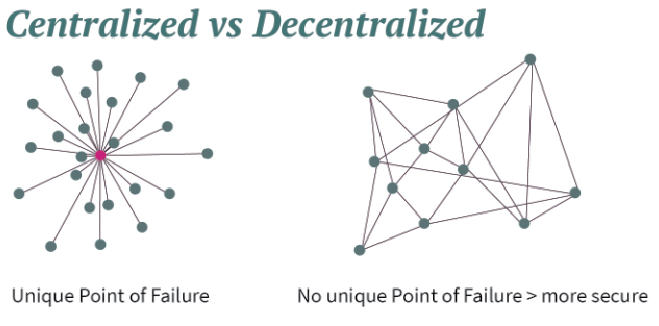
\includegraphics[width=\linewidth]{images/centralized_decentralized}
	\caption{Unterschied zwischen zentraler und dezentraler Architektur~\cite{Blockchainhub.net.2019}}.
	\label{centralized_dezentralized}
\end{figure}


\subsubsection{P2P-Netzwerk}

P2P steht für Peer-to-Peer und bildet im Netzwerk-Kontext das grundlegende Konzept der Dezentralisierung. In einem Peer-to-Peer-Netzwerk sind alle Teilnehmer untereinander gleichberechtigt, wobei jeder Rechner Funktionen, Ressourcen oder Services anbieten oder in Anspruch nehmen kann. Ein \textit{Peer} kann dabei ein einzelner Rechner oder eine Gruppe von Rechnern sein. Ein P2P-Netz kommt ohne Server aus und ist demnach das Gegenteil einer Client-Server-Architektur~\cite{Luber.2018}. 


\subsubsection{Die Blockchain}

Eine wichtige Technologie hin zum dezentralen Web ist Blockchain. Durch die von Satoshi Nakamoto
\footnote{
	Unter diesem Pseudonym wurde im Jahr 2008 das White Paper \textit{Bitcoin: A Peer-to-Peer Electronic Cash System} veröffentlicht, bislang ist unklar ob es sich um eine einzelne Person oder ein Kollektiv von Personen handelt~\cite{BTCAcademy.2018}
}
erfundene Kryptowährung wurde erstmals die Funktion der Währung und damit einhergehend auch der Blockchain erläutert.
Die Blockchain selbst ist eine auf alle Netzwerkgeräte verteilte Datenbank, die sogenannte Blöcke mit Transaktionen enthält~\cite[S. 8]{Crosby.2016}. Diese Transaktionen entstehen zwischen zwei Vertragspartnern und können von jedem Netzwerkteilnehmer verifiziert werden. Für diese Verifizierung wird Rechenleistung benötigt, die von sogenannten Minern für eine bestimmte Vergütung zur Verfügung gestellt wird. Nach der Verifizierung wird die Transaktion in einen Block der Blockchain geschrieben und im Netzwerk distribuiert. Eine Änderung ist ab diesem Punkt nicht mehr möglich, was diese Technik sicher vor Manipulationen und der Abhängigkeit von Vermittlungsplattformen (Intermediären) macht. Wird ein neuer Block hinzugefügt, verweist dieser auf den Hash-Wert des vorherigen Blocks, daher kommt auch der Name \textbf{Blockchain} (zu deutsch: Kette aus Blöcken).

Wie kann jedoch die Sicherheit der Transaktionen garantiert werden? Nun, der Quellcode der Blockchain ist Open Source und daher von allen Nutzern einsehbar. Und darin ist festgelegt, wie mit der Manipulation von einzelnen Transaktionen verfahren wird. Da die verifizierten Blöcke allen Netzwerkgeräten zur Verfügung gestellt werden und somit die "korrekte" Blockchain bekannt ist, werden Änderungen an dieser sofort erkannt und die entsprechenden Geräte aus dem Netzwerk ausgeschlossen. Für eine erfolgreiche Manipulation müssten demnach alle Blockchains auf allen Geräten verändert werden, was schier unmöglich ist.


\subsubsection{Wallet}

Um nun an einem Blockchain-Netzwerk teilhaben zu können, benötigt man ein sogenanntes Wallet. Dies ist eine Software, die bestimmte Algorithmen enthält und auf dem eigenen Client-Gerät ausgeführt wird. 
Um nun an den Vorgängen im Netzwerk teilhaben zu können, werden 2 Keys benötigt: Der Private und der Public Key. 
Der im ersten Schritt generierte Private Key ist ein zufällig-generierter 256-bit Integer, und sollte nicht weitergegeben werden. Er dient dazu, eigene Transaktionen zu signieren. Aus dem Private Key wird im zweiten Schritt mittels \textit{Elliptic-Curve- Cryptography} der Public Key generiert. Diese mathematische Funktion ermöglicht zu jeder Zeit die Ableitung des Public Keys vom Private Key, der umgekehrte Weg (also die Erstellung des Private Keys mittels des Public Keys) würde die leistungsfähigsten Supercomputer mehrere Billionen Jahre beschäftigen. Der generierte Public Key steht auch anderen Nutzern zur Verfügung, und über diesen können Miner verifizieren, ob eine Transaktion tatsächlich von dem Wallet signiert wurde, von dem es vorgibt~\cite[S. 41]{Voshmgir.2019}. 
Aus dem Public Key wird zusätzlich mit einem differenzierten Algorithmus eine Blockchain-Adresse mit Meta-Informationen generiert. Der Algorithmus dient als zweite Sicherungsschicht, für den Fall dass der erste Algorithmus irgendwann mittels Quantencomputern geknackt werden kann. Die Blockchain-Adresse wird wie eine Bankkontonummer verwendet und dient zur eindeutigen Identifikation des Wallet~\cite[S. 42]{Voshmgir.2019}.
Entgegen dem allgemeinen Glauben werden jedoch keine Tokens im Wallet gespeichert. Im Beispiel von Bitcoin heißt dass, das im Wallet keine Bitcoins selbst gespeichert sind. An dieser Stelle ist der Begriff Wallet nicht sehr treffend gewählt, denn darin werden nach dem Private- und Public-Key-Pair alle Transaktionen gespeichert, in denen der Public Key verwendet wurde.
% Beleg (Voshmgir)

Um den Prozess noch einmal abzubilden: Das Wallet (eine Software) enthält Private und Public Key, die Blockchain-Adresse und einige weitere Informationen für spezielle Transaktionen. Zusätzlich werden Einträge gespeichert, die Transaktionen mit dem eigenen Public Key enthalten~\cite[S. 42]{Voshmgir.2019}.
Wird nun eine Transaktion ausgeführt, wird diese auf dem eigenen Gerät mit dem Private Key signiert. Diese signierte Transaktion nennt man \textit{Digital Signature}. Ein anderer Netzwerkteilnehmer kann nun mit der Transaktion und dem Public Key des Senders verifizieren, dass es sich wirklich um denjenigen handelt, der er vorgibt zu sein. Erst nach erfolgreicher Identifikation und Verifizierung wird die Transaktion in die Blockchain geschrieben und an alle anderen Teilnehmer im Netzwerk verteilt. Die Transaktion kann nun nicht mehr verändert werden.

\subsubsection{Smart Contracts}


Smart Contracts sind einem normalen Vertrag ziemlich ähnlich: Zwischen zwei oder mehreren Vertragspartnern geschlossene Vereinbarungen werden darin festgehalten. Dies geschieht jedoch nicht auf Papier, sondern in Form von Programmcode, der in der Blockchain ausgeführt wird. Genau wie die Blockchain selbst ist auch ein Smart Contract Open Source, und auch er kann nachträglich nicht mehr geändert werden. Verträge können somit nicht mehr so leicht verletzt werden. Ein weiterer großer Vorteil ist, dass bestimmte Aktionen automatisch ausgeführt werden können, ohne manuelles Eingreifen zu benötigen. 
Als Beispiel werden oft Lieferketten angeführt: Über die automatische Sendungsverfolgung kann zum Beispiel der Kaufbetrag automatisch überwiesen werden, wenn die Ware beim Kunden ankommt. 
Des weiteren fallen bei Smart Contracts zusätzliche Kosten weg, wie beispielsweise die eines Notars. 
Durch die Dezentralisierung der Verträge ist sichergestellt, dass dieser auch eingehalten wird, und handelsübliche, rechtskräftige Verträge werden nicht mehr benötigt.

Die bekannteste Plattform für die Nutzung von Smart Contracts ist die Plattform \textit{Ethereum}. Diese ermöglicht die Nutzung und Erstellung sogenannter \textit{Dapps}, was für \textit{Distributed Apps} steht (zu deutsch: dezentrale Anwendungen). Durch diese Anwendungen können Smart Contracts erstellt und auf der Blockchain ausgeführt werden~\cite{Ethereum.2019b}. Zudem entstehen zunehmend Anwendungen, die die einfache Erstellung solcher Smart Contracts über eine Oberfläche ermöglichen, sodass auch nicht-Programmierer die Möglichkeit haben, an diesen teilzuhaben.




\subsection{Konzept der Dezentralisierung im Web3}

Doch wie findet nun die Technologie der Blockchain Einsatz in der nächsten Generation des Webs? Da die Blockchain maßgeblich im Zuge der Erfindung der Kryptowährung Bitcoin bekannt geworden ist und diese kontrovers diskutiert wird~\cite{Crosby.2016}, werfen viele die zugrunde liegende Blockchain-Technologie oft mit der Währung in einen Topf. In Wirklichkeit dient sie jedoch für Bitcoin (und andere Kryptowährungen) nur als Mittel zum Zweck, und funktioniert seit deren Einsatz einwandfrei~\cite{Crosby.2016}.
Nichtsdestotrotz denken viele Menschen bei dem Term Blockchain sofort an eine Kryptowährung. Dadurch fällt es schwer, sich auch andere Einsatzgebiete für die Technologie vorzustellen, beziehungsweise wie dieses Konzept aussehen soll. Dazu muss man nun das zuvor erläuterte Konzept der Dezentralisierung mit der Technik der Blockchain in Verbindung bringen: Computer oder Smartphones, wie sie heute bereits in Massen existieren, bilden auf der untersten Ebene die Netzwerkgeräte, die untereinander verknüpft sind. Mit einem darauf aufbauenden Blockchain-Netzwerk können nun verschiedenste Aufgaben erledigt und Dienste angeboten werden, die in Form von den beschriebenen Transaktionen ablaufen. Wichtig dabei ist, dass diese Blockchain-Netze grundlegend auf Tokens aufbauen. Im Beispiel von Bitcoin oder Ethereum sind die Tokens die Währung, in der gehandelt wird. 
Das Bitcoin-Netzwerk nutzt eine gleichnamige Währung (Bitcoin, abgekürzt BTC), im Fall von Ethereum ist die Währung Ether (oder ETH). Tokens sind jedoch ein allgemeines Konzept und unterscheiden sich von Netzwerk zu Netzwerk. 

Tokens sind ebenfalls nicht zwingend eine Währung wie Bitcoin oder Ether, sondern sie können viel mehr Dinge repräsentieren. 
Shermin Voshmgir führt in ihrer Literatur 3 Arten von Tokens an: \textit{Vermögenswerte} (zum Beispiel Strom in Kilowattstunden, Fiat-Währungen
\footnote{
	Fiat-Geld ist eine Währung, die keinen inneren bzw. festen Wert hat, so wie es bei Rohstoffen wie Gold oder Tabak der Fall ist~\cite{CAPinside.2018}. Von Zentralbanken ausgegebenes Geld wie Euro oder Dollar zählen ebenfalls zum Fiat-Geld. 
}, 
Versicherungspolicen oder Event-Tickets), \textit{Zugriffsrechte} (wie Softwarelizenzen, Mitgliedschaften oder Wahlrechte) und eine \textit{Mischform} der beiden (Rechte zum "'minen"' oder native Tokens des jeweiligen Netzwerks (beispielsweise ETH oder BTC)~\cite[S. 151]{Voshmgir.2019}.
Das heißt, dass eben nicht nur mit einer einzigen Währung bezahlt werden kann, sondern viele verschiedene Transaktionen ausgeführt werden können. Manche sprechen sogar von Beispielen, in denen ganze Autos oder Immobilien auf die Blockchain gehoben werden. Dadurch kann beispielsweise ein Testament als Smart Contract aufgelegt werden. Im Todesfall der betreffenden Person wird so das Vermögen auf die Erben verteilt, exakt so wie es im Smart Contract festgehalten ist~\cite[02:10]{Krypto.2018}. 

\smallskip

So wichtig die Blockchain jedoch für das Web3 ist, kann sie allerdings mitnichten als Synonym für den Begriff dienen, wie es ab und zu bei Journalisten oder der Allgemeinheit der Fall ist~\cite[S. 27]{Voshmgir.2019}. Vielmehr ist Blockchain bloß eine Technologie von vielen, die in einem dezentralen Internet Einsatz finden.
Um jedoch den Weg dorthin weitestgehend zu vervollständigen, werden einige andere Protokolle und Techniken benötigt, um die heutigen Dienste mehr oder weniger abbilden zu können. Die Blockchain stellt in diesem Szenario einen großen Nutzen da, um in einem Peer-to-Peer-Netzwerk feststellen zu können, wer was und wann getan hat. Allerdings ist diese nicht dafür geeignet, große Datenmengen zu speichern und zu verarbeiten. Dies hat hauptsächlich 2 Gründe: Erstens sind Blockchains zu langsam und zu rechenintensiv, zweitens bietet die Blockchain nicht immer die richtigen Privatsphäre- und Datenschutzeinstellungen~\cite[S. 27]{Voshmgir.2019}. Zur Größeneinordnung: Die Blockchain des Bitcoin-Netzwerks stieg bis zum dritten Quartal im Jahr 2019 rasant auf eine Größe von knapp 250 GB~\cite{Blockchain.2019}. 

\smallskip

Um nun das Web3 alltagstauglich einsetzen zu können, müssen wenigstens die folgenden Bereiche durch dezentrale Anwendungen abgedeckt werden~\cite[S. 27]{Voshmgir.2019}:

\begin{itemize}
	\item Computerberechnungen
	\item Speicherplatz
	\item Kommunikation und Nachrichtenübermittlung
	\item Monetarisierung
	\item Zahlungsabwicklung
\end{itemize}

Die Blockchain-Technologie kann in diesem Konstrukt mit einem Prozessor in einem Rechner verglichen werden. Er ist für die grundlegende Funktionalität essentiell, benötigt jedoch noch andere Komponenten, ohne die das System nicht anwendbar wäre. 

Mittlerweile gibt es bereits viele dezentrale Anwendungen, die als Lösungen für die oben genannten Komponenten dienen können~\cite{gdamdam.2019}. Viele Protokolle und Plattformen sind noch in der Entwicklung, diese werden jedoch von Zeit zu Zeit besser, indem vor allem zunehmend Unternehmen in diesem Bereich forschen und Entwickeln. Dies belegt vor allem die steigende Zahl der weltweit gegründeten Unternehmen und Start-Ups in dieser Sparte seit 2013~\cite{IPlyticsGmbH.2019}. 

Einige dieser Projekte werden im nächsten Kapitel vorgestellt. Der Fokus liegt dabei darauf, wie diese dezentralen Anwendungen heutige Dienste und Plattformen abbilden oder sogar durch ein neues Konzept ersetzen können. 


\subsection{Dezentralisierung an Alltagsbeispielen erklärt}

Die Beispiele sind in verschiedene Kategorien unterteilt, die allesamt dezentralisiert sind und teilweise sogar aufeinander aufbauen, um eine umfassende Web3-Umgebung zu konzipieren.


\subsubsection{Protokolle und Technologien}

Protokolle und Technologien im Web3 basieren zum Teil auf Blockchain und sollen dabei helfen, verschiedenste dezentrale Anwendungen zu entwerfen und in den Web3-Stack zu implementieren. 


\paragraph{IPFS | InterPlanetary File System}

\begin{figure}
	\centering
	
\includegraphics[scale=0.5]{images/ipfs_logo}
	\caption{Logo des IPFS-Protokolls~\cite{ProtocolLabs.2019}}
	\label{fig:ipfs}
\end{figure}

Das IPFS ist ein Peer-to-Peer-Dateisystem, das den Anspruch erhebt, das HTTP-Protokoll abzulösen~\cite{IdeasEngineering.2018}. In diesem Netzwerk werden Dateien über einen kryptographischen Hash eindeutig identifiziert und auf Netzwerk-Nodes (also einzelne Rechner im Netzwerk) verteilt. Das Konzept orientiert sich dabei an dem Protokoll BitTorrent, das ebenfalls auf den serverlosen Dateiaustausch zwischen Peers setzt. Die Dateien selbst werden jedoch auf jedem der Peers (oder Nodes) in einem Git Repository verwaltet und unterstützen Versionierung~\cite{IdeasEngineering.2018}. Und auch wenn BitTorrent und weitere Protokolle der gleichen Kategorie wie Napster oder KaZaA sehr große Durchsatzraten besitzen, so sind sie dennoch nicht als Infrastruktur ausgelegt~\cite{Benet.2014}.

An diesem Punkt setzt IPFS an, das zwar genau wie HTTP auf TCP/IP aufsetzt, jedoch nicht alleine von diesem Netzwerk-Protokoll abhängig ist. Der größte Vorteil gegenüber HTTP liegt dabei in der Verteilung von vor allem großen Dateien. Diese können sogar in Teilen von verschiedenen Nodes abgerufen werden und sind somit nicht von einer einzigen Bandbreite abhängig. Dieses bietet auch im Streaming enorme Vorteile, vor allem wenn die Datei stark frequentiert ist. Durch das Abrufen eines Videos beispielsweise wird die Datei zur Wiedergabe auf das eigenen Gerät heruntergeladen. Dadurch wird diese jedoch gleichzeitig auch anderen Netzwerkteilnehmern zur Verfügung gestellt, die eventuell sogar geographisch einen kürzeren Abstand besitzen und die Dateien somit nicht mehr um die ganze Welt geschickt werden müssen. Dies funktioniert, da IPFS Inhalte (also Dateien) über deren Hash-Werte adressiert, und nicht wie HTTP über Speicherorte. Wird eine Website über HTTP(S) über einen Domainnamen aufgerufen, wird dieser Name über ein Domain Name System zu einer IP-Adresse und einem Speicherort auf dem adressierten Server aufgelöst. Bei IPFS hingegen sucht sich das Netz bei einem Dateiaufruf die am nächsten gespeicherte Datei, was einen enormen Geschwindig-keitsvorteil darstellt und zusätzlich Ausfallsicherheit gewährleistet~\cite{CodersBlog.de.2019}
Davon abgesehen ist auch ein Dateizugriff möglich, wenn bestimmte Netzwerk-Bereiche durch beispielsweise Zensur oder Naturkatastrophen abgeschnitten sind~\cite{IdeasEngineering.2018}.

\smallskip

\textsc{Sidenote:}
\textit{
	Nachdem die Zentralregierung in Madrid verschiedene Domains hat sperren lassen, die zur Organisation des katalanischen Referendums zur Unabhängigkeit dienten, veröffentlichte der katalanische Präsident Puigdemont einen Link auf eine Datei in einem IPFS-Netzwerk~\cite{Winters.2017}. Da heutige Browser das IPFS-Protokoll noch nicht implementiert haben, muss der Dateiaufruf über einen Webserver auf HTTP umgeleitet werden~\cite{IdeasEngineering.2018}, die Datei selbst mit Informationen über das Referendum am 01. Oktober 2017 war jedoch in einem dezentralen Netz verfügbar.
}


\paragraph{Blockstack}

Blockstack ist ein dezentrales Internet und bietet eine Plattform für die Entwicklung dezentraler Apps und verschiedensten Öko-Systemen. Die beiden Gründer des New Yorker Unternehmens, Muneeb Ali und Ryan Shea, wollen damit gegen die Macht, Einflussnahme und Vorherrschaft der GAFA-Konzerne
\footnote{
	\textbf{G}oogle, \textbf{A}pple, \textbf{F}acebook und \textbf{A}mazon
}
vorgehen~\cite{Kyriasoglou.2018}. Der Schwerpunkt liegt dabei auf Datensicherheit durch Verschlüsselung und Privatsphäre. Da alle Daten verteilt und nicht auf einem zentralen Server gespeichert sind, hat der Nutzer ständige Kontrolle, inklusive der vollständigen Löschung seiner gesamten Daten~\cite{Kyriasoglou.2018}.


\subsubsection{Databases}


\paragraph{BigchainDB}

\begin{figure}
	\centering
	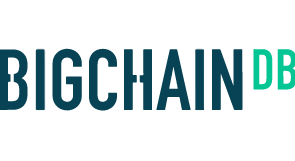
\includegraphics[scale=0.5]{images/bigchaindb_logo}
	\caption{Logo-Schriftzug der Bigchain-Datenbank~\cite{Vecta.io.2019}}
	\label{fig:bigchaindb}
\end{figure}

Die vom Berliner Startup \textit{Ascribe} ins Leben gerufene Datenbank BigchainDB setzt ebenfalls auf die Blockchain-Technologie. Sie soll, wie andere dezentrale Anwendungen auch, "'dezentralisierte Kontrolle, Widerstandsf{\"a}higkeit gegen Manipulationen [sowie] Erzeugung und {\"U}bertragung von Werten"'~\cite{Schmiechen.2016} bieten. Dabei deckt sie ein weitläufiges Einsatzgebiet ab, sowohl für Privatpersonen als auch für Unternehmen. Dazu zählen unter anderem~\cite{Schmiechen.2016}:

\begin{itemize}
	\item \textbf{Verbindliche Verträge} mit allen dazugehörigen Transaktionen können direkt in der BigchainDB gespeichert werden.
	\item \textbf{Erzeugung und sofortige Übertragung von großen Vermögen.} Nur der Besitzer der Vermögen kann diese übertragen. Nicht der Netzwerkadministrator, wie in bisherigen Datenbanksystemen. Kosten werden minimiert, alles soll schneller gehen.
	\item \textbf{Echtzeit-Verfolgung der Produktion von Gegenständen.} Zum Beispiel indem Daten von RFID-Chips in Bigchain gespeichert werden. So sollen Kosten gespart und Betrug vermieden werden.
	\item \textbf{Nachhalten von Urheberrechten.} Digitale Kunstwerke oder Musik kann mit einem Wasserzeichen versehen werden. Alle Informationen über die Verbreitung und Kopien werden dann in der Bigchain gespeichert. Der Lizenzinhaber behält den Überblick über die Verbreitung seiner Werke. Auf dieses Feld hat sich Ascribe konzentriert.
	\item \textbf{Zeitstempel, Zertifikate und Quittungen.} Bigchain ist in der Lage, digitale Vorgänge offen zu legen. Wann wurde was übertragen? Das verhindert juristische Probleme bei Vertragsabschlüssen.
	\item \textbf{Verbesserung der Verlässlichkeit von Datenbanken.} Bis jetzt kann ein einziger Fehler zu Datenlecks führen. BigchainDB kann das verhindern.
\end{itemize}

Der größte Vorteil liegt jedoch zweifelsohne in der Geschwindigkeit: Durch den dezentralen Ansatz soll die Datenbank in der Lage sein, mehr als eine Million Vorgänge pro Sekunde abzuarbeiten. Dies ermöglicht die hohe Skalierbarkeit, die zu Anfang des Produkts nicht gegeben war~\cite{Schmiechen.2016}. 


\paragraph{IPDB | InterPlanetary Database}

Nicht zu verwechseln mit der \textit{Internet Pinball Machine Database} (erreichbar unter ipdb.org) verspricht die Webseite unter ipdb.io eine neue Datenbank für das dezentrale Web. Die von \textit{The Interplanetary Databse (IPDB) Foundation e.V.}, einer deutschen Non-Profit-Organisation, ins Leben gerufene Datenbank baut auf der zuvor beschriebenen BigchainDB und dem IPFS auf~\cite{IPDB.2018}. Das Projekt wird derzeit von einem Konsortium von Organisationen unterstützt, die die Idee einer gut verwalteten Blockchain-Datenbank unterstützen~\cite{IPDB.2018}. Shermin Voshmgir sieht diese Datenbank hauptsächlich im Gebiet der Metadaten-Speicherung in einem P2P-Netzwerk~\cite[S. 29]{Voshmgir.2019}. 


\subsubsection{Datenspeicherung und -freigabe}

\paragraph{Storj}

Diese im Jahr 2014 als Open-Source gegründete Plattform ist die dezentrale Dropbox (oder Google Drive). Storj wird in diesem Fall wie "Storage" ausgesprochen~\cite{Blockchainwelt.2019}. Das in Atlanta ansässige Unternehmen Storj Labs bietet sein Produkt im Prinzip als zweiseitige Medaille an. Auf der einen Seite stehen die sogenannten \textit{Farmer}, die eigenen Speicherplatz bereitstellen und dafür entlohnt werden. Wer nun eigene Dateien in der Cloud speichern möchte, mietet sich dafür einfach Speicherplatz. Dieser Speicherplatz wird jedoch nicht auf einem einzigen Geräte bereitgestellt, vielmehr werden die hochgeladenen Dateien in Fragmente, sogenannten \textit{Shards}, unterteilt und auf viele verschieden Farmer verteilt~\cite{Blockchainwelt.2019}. 

\smallskip

\textsc{Sidenote:}
\textit{
	Ein Farmer in einem Storj-Netzwerk kann auch als Node oder Peer bezeichnet werden. 
}

\smallskip

Hauptaugenmerk bei dieser Anwendung liegt auf der Ende-zu-Ende-Verschlüsselung und die Fragmentierung der einzelnen Dateien. Selbst wenn es einem Angreifer gelingen würde, die Verschlüsselung zu knacken, hätte er nur ein Fragment der Datei, und ohne die Speicherorte der anderen Fragmente kann die Datei kaum gelesen werden. Die Information über die Speicherorte der einzelnen Fragmente besitzt jedoch nur der Eigentümer der Datei, was einen Höchstgrad an Sicherheit garantiert~\cite{Blockchainwelt.2019}.


\paragraph{Sia}

Das Konzept des Speicheranbieters Sia ist dem von Storj sehr ähnlich. Hier besitzt ein Nutzer der Cloud sogar einen eigenen privaten Chiffrierschlüssel. Der Zugriff auf die Dateien erfolgt automatisch mittels einem Smart Contract, was zusätzliche Sicherheit gewährt. Zudem gilt auch hier, dass niemand anderem (vor allem einer fremden Person oder einem fremden Unternehmen) vertraut werden muss, und trotzdem sind die Daten redundant und damit ausfallsicher in der Cloud abgelegt~\cite{Sia.2019}.


\paragraph{Swarm} Diese verteilte Speicherplattform setzt auf dem Web3-Stack der Plattform Ethereum auf, und ermöglicht Entwicklern die Nutzung von redundantem Speicher, etwa für Dapp-Code, Benutzerdaten oder Metadaten zur Blockchain~\cite{Swarm.2019}. Swarm ist Teil der Roadmap von Ethereum hin zu einem dezentralen Internet. Es existiert dabei neben Smart Contracts und Whisper als dezentrale Nachrichtenübermittlung und stellt daher einen essentiellen Part dar~\cite{Gerring.2016}.

% Ggf. weitere Beispiel einfügen

\medskip

Abschließend lässt sich festhalten, dass es eine zunehmende Anzahl von dezentralen Netzwerken und Anwendungen gibt, die mehr oder weniger auf Blockchain basieren. In folgendem GitHub-Repository von \textit{gdamdam} (\url{https://github.com/gdamdam/awesome-decentralized-web}) ist eine Liste von dezentralen Technologien zu finden, die noch immer erweitert wird.



\subsection{Vor- und Nachteile}

\textsc{Recap:} Viele Vorteile des dezentralen Webs wurden bereits in den vorhergehenden Ausführungen angesprochen und erläutert, zur Vollständigkeit werden nachfolgend die Wichtigsten erneut aufgelistet:

\begin{itemize}
	\item \textbf{Ausfallsicherheit:} In einem verteilten Netz gibt es keinen Single-Point-of-Failure, was erhöhte Datenverfügbarkeit in den meisten Bereichen mit sich bringt.
	\item \textbf{Schutz vor Angriffen:} Blockchain-basierte Netzwerke und Anwendungen besitzen viel höhere Sicherheitsmaßnahmen, beispielsweise durch starke Verschlüsselungsalgorithmen. Zudem können Angriffe nicht auf einen einzigen Server konzentriert werden, um beispielsweise Daten zu stehlen oder einen Ausfall zu verursachen.
	\item \textbf{Datenschutz und Privatsphäre:} Nutzer sind Eigentümer über die eigenen Daten und müssen diese keinen Intermediären anvertrauen. Sie haben bei korrekter Anwendung (wie zum Beispiel Geheimhaltung des Private Keys) die alleinige Kontrolle über die eigenen Daten, können frei über diese verfügen und sie gegebenenfalls löschen. Auch der Schutz vor Angriffen bewirkt eine enorme Senkung der Eingriffe in die Privatsphäre der Nutzer.
	\item \textbf{Keine Intermediäre:} Dieser Punkt birgt Vorteile in vielen Bereichen. Durch den Wegfall der Vermittlungsplattformen können enorme Kosten und Wege gespart werden, dies zudem bei höchstem Datenschutz.
	\item \textbf{Smart Contracts:} Bereits heute gibt es eine Vielzahl von Anwendungsfällen, die viele Vorgänge einfacher und sicherer gestalten können. Diesen ist nach oben hin keine Grenze gesetzt, und Smart Contracts haben die Möglichkeit, sowohl das Privatleben als auch die Prozesse von Unternehmen massiv zu verändern.
\end{itemize}

\smallskip

Diese Punkte jedoch so stehen zu lassen, wäre nicht korrekt, denn die Entwicklung dieser Protokolle und Anwendungen hat quasi gerade erst begonnen. Durch den Anstieg an Unternehmen, die sich in diesem Bereich angesiedelt haben, stehen mehr und mehr Ressourcen für Forschung und Entwicklung zur Verfügung, dennoch müssen viele Probleme erst noch gelöst, geschweige denn erkannt werden. Und auch wenn es für viele der heutigen Anwendungen bereits dezentrale Lösungen gibt, fehlt es dennoch an einer Auswahl an etablierten Netzen und Plattformen, um einen produktiven Einsatz zu gewährleisten. 

Des Weiteren steht und fällt eine Anwendung mit ihrer Programmierung. Auch wenn Bugs heute bereits fatale Folgen haben können, ist die Entwicklung mit bekannten Techniken in den allermeisten Fällen serienreif, und immer beliebter werdende Test-Frameworks und -Prozesse sichern die korrekte Ausführung der Programme. Da viele dezentrale Projekte den Open-Source Ansatz verwenden, greift in diesen Fällen das Vier-Augen-Prinzip, was die Fehlersuche beschleunigen kann. Dennoch werden dafür auch genügend Entwickler benötigt, die dieser Aufgabe nachkommen und die dafür qualifiziert sind. 

Vor allem bei den Smart Contracts können Programmierfehler ein hohes Risiko bergen. So verlässlich und automatisiert sie in ihrer Ausführung sind, so sicher werden eben auch Probleme bei falscher Programmierung verursacht, wie das folgende Beispiel zeigt.

\smallskip

Dem Wagniskapitalgeber \textit{The DAO}, der im April 2016 mit 150 Millionen US-Dollar aus einer Crowdfunding-Kampagne startete, wurde dies zum Verhängnis. The DAO war eine \textbf{d}ezentrale, \textbf{a}utonome \textbf{O}rganisation (daher der Name), die mithilfe von Smart Contracts in Unternehmen, vor allem in Start-Ups investieren wollte. Der Unterschied zu anderen Venture-Capital-Firmen? Die Organisation kommt ohne Management oder Direktoren aus, stattdessen werden die Entscheidungen für Investitionen automatisch mit Smart Contracts getroffen~\cite{Reiff.2019}.
The DAO setzte auf Ethereum auf und benutzte dessen Währung ETH. Bereits im Juni des selben Jahres gelang es jedoch einem Nutzer, über einen längeren Zeitraum insgesamt Ether im Wert von ungefähr 50 Millionen US-Dollar auf sein eigenes Konto umzuleiten~\cite{Reiff.2019}. Während die Gründer überlegten, wie sie das Geld zurückholen können, bekamen sie einen Brief des "Diebs", und darin drohte dieser The DAO mit rechtlichen Schritten! Er gelangte nämlich durch einen Programmierfehler eines Smart Contracts an die Tokens, und auch wenn sein Verhalten unethisch war, illegal war es nicht~\cite[05:08]{Krypto.2018}. Letztendlich erhielt er das Geld nicht, dennoch führte der "Diebstahl" bereits im September 2016 zum Ende von The DAO~\cite{Reiff.2019}. 

Das Ethereum-Netzwerk wurde einem Hard-Fork unterzogen. Das heißt es gibt derzeit 2 Versionen von Ethereum: Eine alte, in der der Programmierfehler immer noch existiert, und eine neue, wo der Fehler durch Updates der Ethereum Nodes behoben wurde. Und obwohl die Ethereum-Community mehrheitlich für den Hard-Fork gestimmt hatte, spaltete der Vorfall die Nutzerschaft, denn dieser sei nicht im Sinne eines führerlosen und dezentralen Systems~\cite{Hayes.2016}. 





